\chapter{Development of Pre-Arcus}
\label{chapter:prearcus}

\begin{quote}
``When I am working on a problem I never think about beauty. I only think about how to solve the problem. But when I have finished, if the solution is not beautiful, I know it is wrong.'' \\
--- \textit{Buckminster Fuller (1895-1983)}
\end{quote}

\section{Introduction}

Following the execution of the \textsl{ConformerBuilder}, described during chapter \ref{chapter:reduced_rep}, a text-file containing all valid conformers for a given loop will have been produced.
These all represent \mainchain\ conformations extending away from the N-terminal anchor. All, by definition, have C-termini close to the C-terminal anchor, but of course will not meet perfectly. Each of these \mainchain-only conformers must now be re-evaluated
after being re-built in all-atom mode. 

This chapter begins with a definition of how ``broken'' coarse-resolution conformers are manipulated under a torsional refinement system. The all-atom models which are produced by this process have been re-joined and are sterically-competent. This level of the build-hierarchy is termed stage 2. Following this, all conformers which could be successfully joined
within tolerances are passed to stage 3, which performs refinement under a more sophisticated forcefield.
Both these stages are described in more detail in the remainder of this chapter.

\section{Torsional Energy Minimisation}

The following section describes the implementation of a steepest-descent energy minimisation protocol,~originally developed by Allan Brewer\cite{THESIS:BREWER}, which operates in torsional space. In this implementation, the \mainchain\ and \sidechain\ single-order bonds within the system, which were originally illustrated in figures \ref{fig:intro:bb_torsion} and \ref{fig:intro:chi} respectively, are  rotated under the control of \emph{Cartesian} forces. Analytical derivation of the energy-gradient with respect to a torsional system is both computationally and mathematically challenging. The use of Cartesian forces both simplifies this and ensures that the minimisation protocol is instantly applicable to all modern molecular mechanics \forcefields. One minor caveat,  is that all forces must be independent of the absolute orientation of the system -- that is, if the entire system is rotated, as a single rigid-body in space, the relative forces on each individual atom must not change; the rationale for which is defined below.

\subsection{The Advantages of Torsional Representation}

Utilisation of a torsional representation results in a drastic reduction of the number of degrees of freedom for a given system. Such simplification, therefore, also yields an implicit reduction in computational complexity and thus a complementary reduction in the required time for simulation. In this dissertation, section \ref{section:protein_rep} has already discussed that a reduction in the degrees of freedom can smooth the potential energy landscape and therefore simplify the search process; but with the caveat that over-simplification is detrimental to the description of the native-state.
Idealised-geometry torsional systems which operate in continuous space generally, however, show very close structural correspondence with their Cartesian counterparts. Indeed native-like states may be generated, which exhibit essentially no deviation from the true native, state solely using idealised geometry.

In Cartesian systems, due to the use of harmonic bonding-terms, small deviations from equilibrium distances  can yield gross changes in ascribed potential energy. As torsional movements cause no deviation from idealised-geometry, the bond and angle energetic terms may be omitted from the forcefield calculations during simulation. 
The torsional system can therefore be thought of as completely neglecting the high-frequency bond and angle oscillations. This is not, however, necessarily detrimental to a simulation. Not only is this omission computationally favourable, but it has also been suggested that the representation
used for standard molecular mechanics is too flexible, because the hard degrees of freedom should really be considered as quantum mechanical oscillators\cite{NATIVE:InternalVibrations}. It is thought that such over-flexibility could also facilitate the inappropriate traversal of torsional barriers. It is also true that, following a typical Cartesian energy minimisation, the deviations found in bond angles when compared to their equilibrium values, is in excess of what would normally be found in peptide crystals\cite{SIMULATION:Gibson90}.


When under torsional control, as compared to Cartesian systems, far larger movements are possible during simulations performed using standard molecular mechanics \forcefields. The step-size is crucial as it fundamentally determines the overall speed of simulation. During standard molecular dynamics and energy minimisations small Cartesian changes are required. At each iteration, if atoms take too large a step, the resultant increase in hard-sphere repulsion energies and bonded-energy terms causes very large attractive and repulsive forces which attempt to reposition the atoms. This force is then equated to further larger atomic movements in the following time-steps, which ultimately creates positive-feedback, resulting in simulation instability.
Under Cartesian MD,\ this difficulty can be alleviated to some extent by one of a number of restraint algorithms derived from \textsc{Shake}\cite{SIMULATION:SHAKE}. All of these ensure that large Cartesian movements, especially in hydrogen atoms, do not occur per-step, but can at best still only realistically facilitate time-steps of up to 2 fs. By equating Cartesian forces to torsional movements, such concerted and large Cartesian movements are avoided.
Recently a torsional system called ICM\cite{SIMULATION:ICM} -- Internal Coordinate Modelling --  has been shown to be up to an order of magnitude faster than MD and can use a time-step of up to 10 fs.
The benefits of such a speed increase are obvious.

\subsection{Implementation}

The algorithm, originally implemented in Visual Basic, was ported during this work. The re-written pure-\CPP\  implementation was  crafted within the \pd\ framework using a more generic code structure. It can now be used in combination with any of \pd s forcefields that define Cartesian first-derivatives of the potential energy for each atom.
In addition to increased generality, it is widely accepted that \CPP\ yields significant additional performance benefits over Visual Basic, when compiled under any modern compiler. 

\subsection{The Mathematical Derivation}

This section is described in relation to figure \ref{fig:prearcus:vector_maths}, which shows mathematical vectors relating to the rotation around an atomic bond, illustrated by a $\Phi$ \mainchain\ torsion angle. In the remainder of this section the $\Phi$ angle will be referred to by $\theta$; a generic term representing any rotatable bond. In this example, the affected atom $k$ is directly bonded to $j$, although this need not be the case; each atom $k$ will be affected by the rotation of around the bond $\vec{ij}$ if there is any non-circular path of covalent bonds joining it to either \mbox{atoms $i$ or $j$}.

For the discussion below,  the atoms $i$, $j$ and $k$ are defined to lie in the plane of the page, each with a z-axis coordinate of zero. Thus, any rotation around the bond $\vec{ij}$ will cause atom $k$ to leave the plane of the page.
In the standard right-handed coordinate system and IUPAC conventions, a positive $\Delta\theta$ is defined as a clockwise rotation and a subsequent outward motion from the page, with a positive value on the z-axis.

\begin{figure}[hptb]
\begin{center}
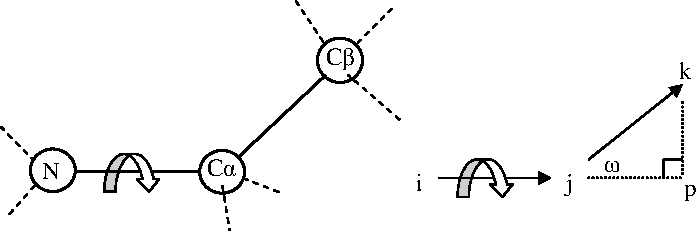
\includegraphics[width=0.8\textwidth]{./06-PreArcus/torsional/definition_reference.pdf}
\end{center}
\caption[Reference diagram for torsional derivation.]{Reference diagram for torsional derivation. (Figure adapted from\cite{THESIS:BREWER}.)}
\label{fig:prearcus:vector_maths}
\end{figure}

The direction of any vector product is perpendicular to the plane formed by the two individual vectors. Thus, the vector product of $\vec{ij}$ and $\vec{jk}$  gives the direction of atom $k$ following an infinitesimal change in the torsion $\theta$. $\left\vert \vec{kp} \right\vert$ is defined as a perpendicular dropped from the position of $k$ to the point $p$, which forms a right-angle with the extrapolation of the vector $\left\vert \vec{ij} \right\vert$.
The relative magnitude of any movement is proportional to $\left\vert \vec{kp} \right\vert$. This statement results from the fact that $\left\vert \vec{kp} \right\vert$ is the radius of a circle, defined by the path of atom $k$ during a complete rotation of the bond $\vec{ij}$. The circumference of such a circle will evidently be $2\pi  \left\vert \vec{kp} \right\vert$, so any angular change will be a fraction of this and therefore, by definition, proportional to $\left\vert\vec{kp}\right\vert$.

By mathematical law, the magnitude of any vector product is calculated as the product of the magnitudes of the vector lengths and the sine of angle between them. Thus,

\begin{equation}
\left\vert \vec{ij} \otimes \vec{jk} \right\vert = \left\vert \vec{ij} \right\vert  \left\vert  \vec{jk} \right\vert \sin\omega 
\end{equation}
and by trigonometry,
\begin{equation}
\sin\omega = \frac{ \left\vert \vec{kp} \right\vert }{ \left\vert \vec{jk} \right\vert }
\end{equation}
it follows that,
\begin{equation}
\left\vert \vec{kp} \right\vert = \frac{ \left\vert \vec{ij} \otimes \vec{jk} \right\vert }{ \left\vert \vec{ij} \right\vert }
\end{equation}

Thus, the magnitude of the rotation around the bond is proportional to the magnitude of the vector product divided by the bond-length between atoms $i$ and $j$, which is a known constant when using idealised-geometry.

We must now consider the magnitude of the movement in the position of atom $k$ with respect to a Cartesian force imposed on that atom, $\vec{F_k}$. The force on atom $k$ must be reconciled with other forces to yield a value for the rotation about the vector $\left\vert \vec{ij} \right\vert$. The  dot product is used here since it returns a scalar quantity which is representative, both of the vector magnitudes and the agreement of their directions. Thus,

\begin{equation}
\Delta\theta \propto \frac{ \left ( \vec{ij} \otimes \vec{jk} \right ) \bullet \vec{F_k} }{\left\vert \vec{ij} \right\vert }
\end{equation}

To complete the primary equation, we must introduce two further terms. The first is a bonding term $B_{k,i}$, which defines the relative side  of the bond from atom $i$ to atom $j$, on which atom $k$ resides. This is a constant taking the value $\pm 1.0$ and defines the direction of the desired rotation. The second is an angular step-size constant $P$ which scales the final magnitude of the rotation. The final torsional change is then defined by the sum over all $k$ atoms.

\begin{equation}
\Delta\theta =P\sum_k B_{k,i} \left( \frac{ \left( \vec{ij} \otimes \vec{jk} \right) \bullet \vec{F_k} }{\left\vert \vec{ij} \right\vert } \right)
\label{eqn:prearcus:primary_torsional}
\end{equation}

The calculation can then be repeated for each active torsion, usually including all rotatable \Chi-angles and the \mainchain\ \phipsi\ pairs with the \Omg-torsion if desired.
The overall calculation is highly computationally efficient, requiring only 10 multiplications and 8 additions per iteration. None of the more expensive computational calls such as trigonometric or exponential functions are required, meaning that the cost of minimisation is usually dominated by the cost of the calculation of forces.

\subsection{Logical Rigour}

It is logically clear that the resolution of forces between an interacting atom pair only affects the rotatable bonds within the covalent path between the two atoms; these are the only bonds that, when rotated, are capable of affecting the relative orientation of the interacting atomic pair. For the calculation to be applicable to any forcefield which supplies net per-atom forces and in order for the torsional minimisation to be as efficient as possible, all forces need to be considered on a per-atom, rather than a pairwise basis. For equation \ref{eqn:prearcus:primary_torsional} to retain rigor, for atoms outside this range, the per-atom forces are required to result in a net zero angle-change for each bond between the pair of atoms. This logically holds true for all force calculations which involve only pairwise distance calculations between atoms\cite{THESIS:BREWER}. These calculations  must, by definition, result in equal but opposite forces on the interacting atoms.
Therefore, the only difficulty is for forcefields which use an interaction field which is not constant for all positions in space. An example of such a forcefield would be an implicit lipid membrane, where re-orientation within the membrane and surrounding implicit-solvent, would alter the relative forces on individual atoms.

\subsection{Selection of ``k'' atoms}

As described in the previous section, it is clear that when considering pairwise forces, the net forces between atoms on either side of the bond must be equal but opposite. It therefore follows that calculating the torsional change for the atoms on one side of the bond will produce an equal, but opposite value to that calculated when considering the atoms on the other side. In light of this, it is always more computationally efficient to consider the side of the bond with fewer atoms. For \Chi-angles this is obviously always the \sidechain. This practice yields a reduction in calculation volume for \Chi-angles from $O(N^2)$ to $O(N)$, whereas the backbone remains $O(N^2)$, reduced by a factor of approximately 4.0 depending on the exact number residues  and atoms per residue.\ 

\subsection{Angle-change Normalisation and Adaptive Step-multiplier}

During the torsional minimisation, large angle-change values can be obtained due to large individual forces. It is, therefore, advantageous to introduce a maximal per-step angle-change. Normalisation is the preferable choice, both because crude capping would alter the relative magnitudes of the calculated angle changes and because towards the end of the minimisation, when the energy gradient is low, the rate of conformational change is maintained.
This normalisation is achieved by modulating the value of
of $P$ with respect to the current energy gradient.

A typical minimisation protocol normally adopts the following logic:

\begin{enumerate} \isep
\item Calculate potential energy of the system and the forces acting upon each atom. 
\item Compare the energy with that of the previous iteration. If the energy gradient is negative, multiply the step-multiplier by 1.2 and store as the lowest-energy conformation state yet visited; otherwise multiply it by 0.5 and retract the move.
\item Goto 1 until the energy gradient falls below cut-off, the maximum number of iterations is reached, or a maximum number of energy-increasing steps is performed.
\item Restore the lowest energy structure visited.
\end{enumerate}
Using an adaptive step-multiplier has the desirable effect of rapidly accelerating along well defined energy gradients and quickly backtracking as the potential energy increases.
It is also true that without such adaptation, the final state of a minimisation will be an oscillation at the bottom the local energy-well.

The procedural call, to retract conformational-changes which increase the potential energy of the system, is required during \emph{Cartesian minimisation} and improves the behaviour of the protocol.\ In fact such retraction is part of the true definition of an energy minimisation. One algorithmic alteration for \emph{torsional systems,} which was empirically found to result in a lower final energy, was to disable this structural reversion. As a result, the torsional energy minimisation used in this work, whilst still reducing the step-multiplier by 0.5 when the energy gradient is positive, does not revert the conformation to the previous lowest energy conformation. In doing this, the protocol ``oversteps'' the local energy minimum by adding ``thermal motion''. This feature can prevent the minimisation becoming trapped in local minima and potentially allows descent to deeper minima. It is noted that this procedure is therefore, not a true minimisation, but takes the place of such a protocol during protein simulation. This practice has been empirically shown, to result in lower energy minima, following minimisation when compared to the  Cartesian conjugate-gradient alternative\cite{THESIS:BREWER}.
The behaviour of the protocol can be \emph{approximately} thought of as performing simulated annealing.

\section{AMBER Modifications}

Many of the standard \forcefield\ calculations involve pairwise calculations between atoms.
It follows that the total calculation time is closely related to the number of atoms in the system. Thus, by reducing the number of atoms, total calculation time may be decreased.
For all \forcefield\ evaluations performed by \prearcus, a modified version of \amberff\ was used, which has no aliphatic hydrogen atoms. All bonded-\forcefield\ terms relating to these hydrogen atoms are also removed from the system. All \mainchain\ and polar hydrogen atoms  were retained, as they are important for electrostatic interactions.
This \forcefield\ has been previously assessed and found to have similar success to the official \amber\ \forcefield\  in folding the TrpCage mini-protein \cite{THESIS:BREWER}. By using this modified forcefield, for a typical modelling run, a speed increase in excess of 4$\times$ is typically obtained.


\section{The Perturbation Scheme}

Three perturbation types are used throughout the \prearcus\ refinement process. Each perturbation is applied in order, where the exact ordering is important. The first perturbation is of the \phipsi\ \mainchain\ torsions. In this case, the \Omg-torsion is not explicitly perturbed, but can move during the refinement protocol. The magnitude of each perturbation is normally distributed, as illustrated in figure \ref{fig:prearcus:pert_mag}, where the parameter $\sigma$ defines the point at which the \first\ standard deviation of the distribution lies.
From the definition of the normal distribution, 68\% of the perturbations will be less than $\sigma$ in magnitude, 95\% under $2\sigma$ and 99.7\% under $3\sigma$.

\begin{figure}[hptb]
\begin{center}
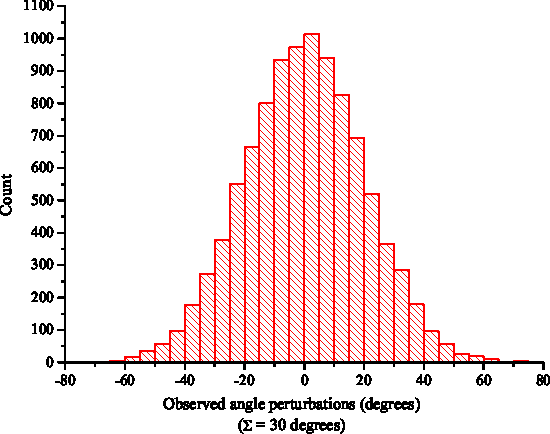
\includegraphics[width=0.7\textwidth]{06-PreArcus/sidechain/sidechain_pert_mag.pdf}
\end{center}
\caption{\Sidechain\ perturbation magnitudes.}
\label{fig:prearcus:pert_mag}
\end{figure}

The second perturbation was used to semi-randomly apply rotameric states to each loop residue in turn. First of all, the steric interactions for the \emph{current conformation} of each residue is assessed by hard-sphere overlap. If the steric score is poor then a rotamer change is forced. If not, then by a user-defined probability, one of two outcomes occurs. A random number of uniform distribution between 0.0 and 1.0 is generated. If this number is under the fractional probability, the
current residue state is kept and the function exits, if not then a change in the rotameric state occurs. Next, the steric environment is assessed for all rotameric states. All those which are under a cut-off are flagged as valid. A random selection is then made from these valid rotameric states.
If no states are valid, then an arbitrary state is chosen entirely at random.

The final perturbation is a \sidechain\ torsional perturbation which is invoked on all loop residues in turn. Each rotatable $\chi$-torsion is perturbed in the same manner as the \mainchain\ torsions, but using a separate value for $\sigma$. A second minor difference is that there is a random probability that, instead of a $\sigma$-dependent rotation, a simple $\pm$120\degree\ flip can occur. This is to ensure that it is possible to cross the rotational barriers between the distinct gauche--, gauche+ and trans rotational states.



\section{Loading Conformers from Stage 1}

Each of the conformers, found to be viable in stage 1, are loaded from a text-file into memory using a class called the \textsl{ConformerBuffer}, itself a type of \textit{\textsl{ConformerBuilder}}. For each iteration of stage 2, the \textsl{ConformerBuffer} applies the next conformer in its list.
This time the builder is set to all-atom mode rather than building only \mainchain\ atoms.

\section{Stage 2: Conformation Re-join}

The specific components of stage 2 are described in this section, followed by a flow-diagram illustrating the execution logic.

\subsection{The Tweak-Generator}

One problem with a reduced model in torsional-space is that small deviations at the beginning of the conformer can result in gross Cartesian changes at its end -- here we term this the ``lever-effect''. Due to this, many conformers which are close to the native in torsional space, may not be in a viable conformation with respect to the steric and end-join filters. In an attempt to optimise these parameters prior to the refinement process, the tweak-store was implemented.
This store, for each given conformer, makes $n$ torsional perturbations for the first $m$ rotatable torsions. For this research, $m$ was defined as the \phipsi\ torsions for the first three residues. The applied tweaks for these initial torsions were the original angle and four torsional tweaks over a $\pm$5.0\degree\ range.
For each of the possible tweaks, the end-join distance and steric-filters defined in stage 1, were measured and the best-scoring tweaked-conformer kept for the refinement process.




\subsection{An Energy Function for Loop Re-join}
\label{section:prearcus:rejoin_force}

A suitable restraining potential for molecular minimisation and dynamics must have a number of distinct properties. As the loop-join potential will be required to act over long distances, something simple like a harmonic-potential will be inadequate. Outside typical equilibrium separations for bonded atoms, the calculated potential energy would be of excessive magnitude, greater than computational precision.  The resultant forces derived during dynamics would be of astronomical sizes and so at best the simulation would be highly unstable. This is to be expected, as harmonic bonded-terms are not designed to accommodate such long bond-lengths.

What is required, is a ``soft'' potential to draw the relevant particles to their desired locations without the calculation of excessive force magnitudes. A linear function would lend itself to this, being of only moderate force at long distance. The difficulty with the use of a linear function comes when two lines of opposite gradient are summed to create an energy-minimum at a given separation; At the point of intersection, a ``singularity'' is created where, mathematically, no first differential is defined. This is a problem during molecular dynamics where continuous differentials are required for the calculation of the forces acting on the particles at all separations. The solution to these two problems is a hybrid equation (\ref{equation:prearcus:rejoin}), which is based on a linear equation, but which decays to zero at a given particle separation. 

\begin{equation}
\text{Potential Energy} = \epsilon\gamma\ln\left(1+\exp\left(\frac{\beta\left( d - d_{\text{Ideal}} \right)}{\gamma}\right)\right)
\label{equation:prearcus:rejoin}
\end{equation}

By summing two potentials of opposite orientation, the result is a linear descent into a smooth flat-bottomed energy well, the shape of which can be varied by a set of four parameters (figure \ref{table:prearcus:rejoin_param_variation}). 
\begin{figure}[htbp]
\begin{center}
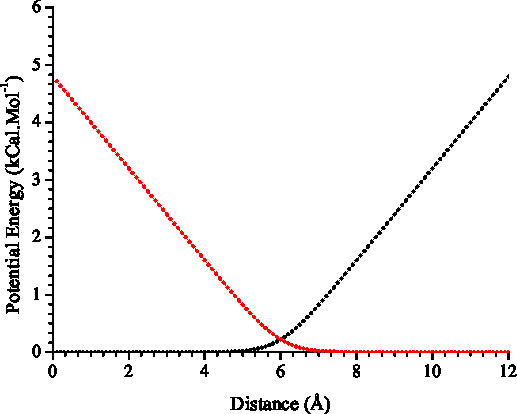
\includegraphics[width=0.68\textwidth]{./06-PreArcus/img/rejoin_dualarm.pdf}
\vspace{0.3cm}
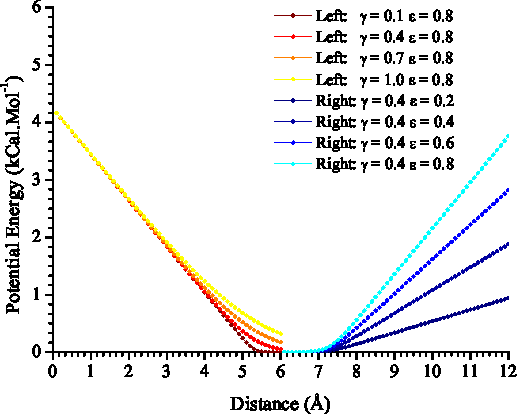
\includegraphics[width=0.68\textwidth]{./06-PreArcus/img/rejoin_params.pdf}
\begin{tabularx}{0.90\textwidth}{+l^X^c^c}
\toprule 
\rowstyle{\bfseries} \multirow{2}{*}{Term} & \multirow{2}{*}{Description} & \multicolumn{2}{c}{\bf{Example Values}} \\
\rowstyle{\bfseries} &  &   Left   &     Right \\
\midrule
Epsilon ($\epsilon$) & Linear slope gradient & 0.8 & 0.2 to 0.8 \\
Gamma ($\gamma$)     & Rate of curve flattening & 0.1 to 1.0  & 0.4 \\
Beta ($\beta$)       & Designated to be $\pm$1.0 only, allowing mirroring of the curve & -1.0 & 1.0 \\
d\subscript{Ideal}   & Alters the point at which the curve decays to zero & 5.3   &  7.3 \\
\bottomrule
\end{tabularx}
\caption[Parameter variation of the constraint well]{Parameter variation of the constraint well. The range of parameters used to create the curves are shown in the accompanying table.}
\label{table:prearcus:rejoin_param_variation}
\end{center}
\end{figure}

In this implementation, when both arms of the well are considered, four user-variable parameters remain for the definition of the overall well-shape (figure \ref{fig:prearcus:rejoin}). The ideal-distance is obviously set on a per-pair basis, leaving the other three parameters as truly variable. For simplicity, although the value of gamma can be varied, a value of 0.4  has been used throughout this work following brief testing (data not shown). Essentially, the value of gamma was shown to have little effect on the end result of restrained MD simulations, the result being dominated by the value of epsilon and the well-width.

\begin{figure}[htbp]
\begin{center}
\begin{tabularx}{0.77\textwidth}{+l^X^c}
\toprule
\rowstyle{\bfseries} Term & Description  &   Example Values \\
\midrule
Well-width & The displacement magnitude for the dual-curves & 1.0 to 3.0 \\
d\subscript{Ideal}  & The d\subscript{Ideal} equation parameter for each arm is defined as this value $\pm$ the well width  &   6.3 \\
Epsilon ($\epsilon$) & Absolute linear slope-gradient & 1.0 \\
Gamma ($\gamma$) & Rate of well-flattening & 0.4 \\
\bottomrule
\end{tabularx}
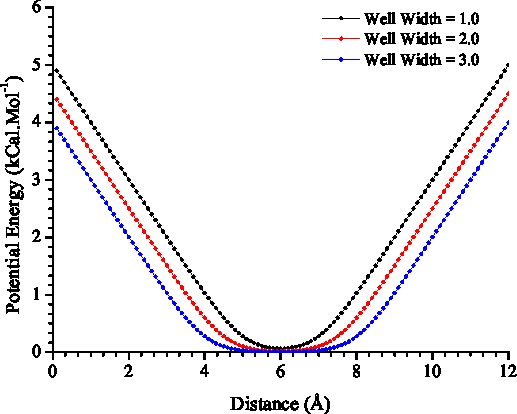
\includegraphics[width=0.65\textwidth]{./06-PreArcus/img/rejoin_well.pdf}
\end{center}
\caption{The user-definable variables of the symmetric v-shaped constraint.}
\label{fig:prearcus:rejoin}
\end{figure}

The flat-bottom is also of importance, as it means that once the restraint is satisfied during dynamics, the contribution to the potential-energy of the system is effectively zero. The width of the flat section can be varied with a ``certainty factor'' for a given restraint -- i.e. restraints with lower certainty would use a well shape with a wider bottom to allow a greater spread of allowed distances. Overall, this means that the potentials can be used to guide an atom-pair to a desired separation, but once the separation is achieved, the forces dictating conformation are those of the physicochemical forcefield alone.

In conclusion, this constraint definition is highly versatile and ideal for this application. The only drawback is the level of computation required, as each of the division, Exp and Ln calls are  computationally expensive when compared to both multiplication and addition. This is, however, unimportant for this application, as only two of these calculations are required to facilitate re-joining. The computational cost of this is, therefore, dwarfed by the other pairwise energy calculations.

\subsection{Perturbation Magnitudes and Forcefield Configuration}

For stage 2, the $\sigma$ for
\mainchain\ perturbations was set as 0.22 radians per torsion.
As described previously, this sets the  value of \first\ standard deviation in a normal distribution. Thus, approximately 68\% of angle perturbations are \mbox{$<$12\degree} and 95\% are \mbox{$<$22\degree}.
Although these magnitudes are under the required 60\degree\ stated in section \ref{section:reduced_rep:subsequentrefinement}, the rotations are cumulative during the refinement process and can also change freely during torsional-minimisation as required. The equivalent term for \Chi-torsion perturbation was set to 0.5 radians, with a 5\% probability per-residue that a 120\degree\ flip would occur instead.
The rotamer perturbation was applied with a 100\% probability per residue.

The \forcefield\  for steric minimisation contained only the \amberff\ torsional terms, the soft-sphere steric forcefield described in figure \ref{fig:db:softvdw} and the loop-join force described in section \ref{section:prearcus:rejoin_force}.

\subsection{Control Logic}

The logic used in stage 2 is illustrated, in general terms in figure \ref{fig:prearcus:stage_2}. The exact protocol  was implemented as follows:

\begin{enumerate} \isep
\item Load the next conformer from the stage 1 list until exhausted.
\item Apply the tweak-generator and keep the single best
found, scored by the stage 1 join-distance and steric score criteria.
\item For $n$ repeats ($n$ set as 5).
        \begin{enumerate} \isep
        \item Apply the \mainchain\ torsional perturbations.
        \item If join-dist $>$ 2.0, goto (a) up to 500 times, else goto (g).
        \item Apply the rotamer-perturbations.  
        \item Apply the \sidechain\ perturbations.
        \item Execute a torsional-minimisation under the steric-forcefield.
        \item If the potential energy of the system is below a conservative \mbox{15,000 \kcalmol}, store the structure.
        \item Restore the best-state from the tweak-generator, then goto a).
        \end{enumerate}
   \item Goto 1.
\end{enumerate}

\begin{figure}[htbp]
\begin{center}
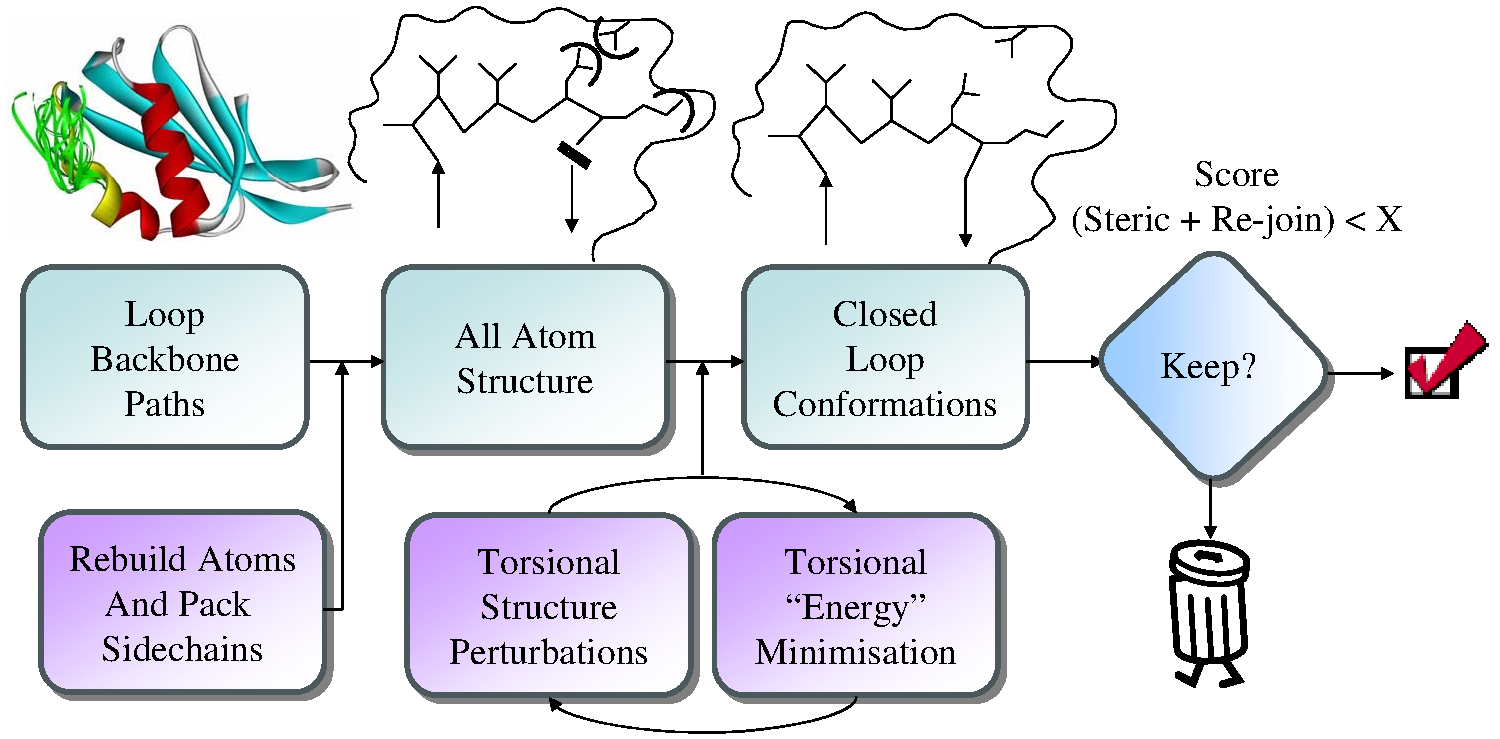
\includegraphics[width=0.9\textwidth]{./06-PreArcus/stage-2/stage-2.pdf}
\end{center}
\caption{The execution logic for \prearcus\ stage 2.}
\label{fig:prearcus:stage_2}
\end{figure} 

\section{Stage 3: Conformation Refinement }

The specific components of stage 3 are described in this section, followed by a flow-diagram illustrating the execution logic.

\subsection{Perturbation Magnitudes and Forcefield Configuration}
\label{section:prearcus:stage3_refinement}

For stage 3, the $\sigma$ for
\mainchain\ perturbations was set as 0.04 radians per torsion.
Again, this gives approximately 70\% of angle perturbations \mbox{$<$2.3\degree} and 95\% are \mbox{$<$4.6\degree}.
The equivalent term for \Chi-torsion perturbation was set to 0.2 radians, with a 1\% probability per-residue that a 120\degree\ flip would occur instead.

Two forcefields were used during stage 3. The first was the full-torsional forcefield, which included the \amberff\ torsional terms, the loop-join force previously described in section \ref{section:prearcus:rejoin_force}, VDW forces and the electrostatic and solvation  terms calculated by the GB \forcefield\  as described in section \ref{section:protmodel:implicit_solvation} and the SASA \forcefield.
The second Cartesian-\forcefield\ used the same terms, \emph{except} for the re-join force and added the remaining standard \amberff\ bonded-terms.

\subsection{Control Logic}

The logic used in stage 3 is illustrated, in general terms, by figure \ref{fig:prearcus:stage_3}. The exact protocol  was implemented as follows:
 
\begin{enumerate} \isep
        \item Load the next structure selected by stage 2.
        \item For $n$ repeats ($n$ set as 15).
        \begin{enumerate} \isep
        \item Apply the \mainchain\ torsional perturbations.
        \item Apply the \sidechain\ perturbations.
        \item Execute a torsional minimisation under the full torsional-forcefield.
        \item If the re-join failed, goto 2.
        \item Execute a conjugate-gradient Cartesian minimisation under the full Cartesian-\forcefield.
        \item Append to the trajectory, for later analysis.
        \item Store the structure and energy. If the best energy visited, store as the best single conformation found.
        \item Restore the structure to that selected by stage 2.
        \end{enumerate}
        \item Goto 1.
\end{enumerate}

\begin{figure}[htbp]
\begin{center}
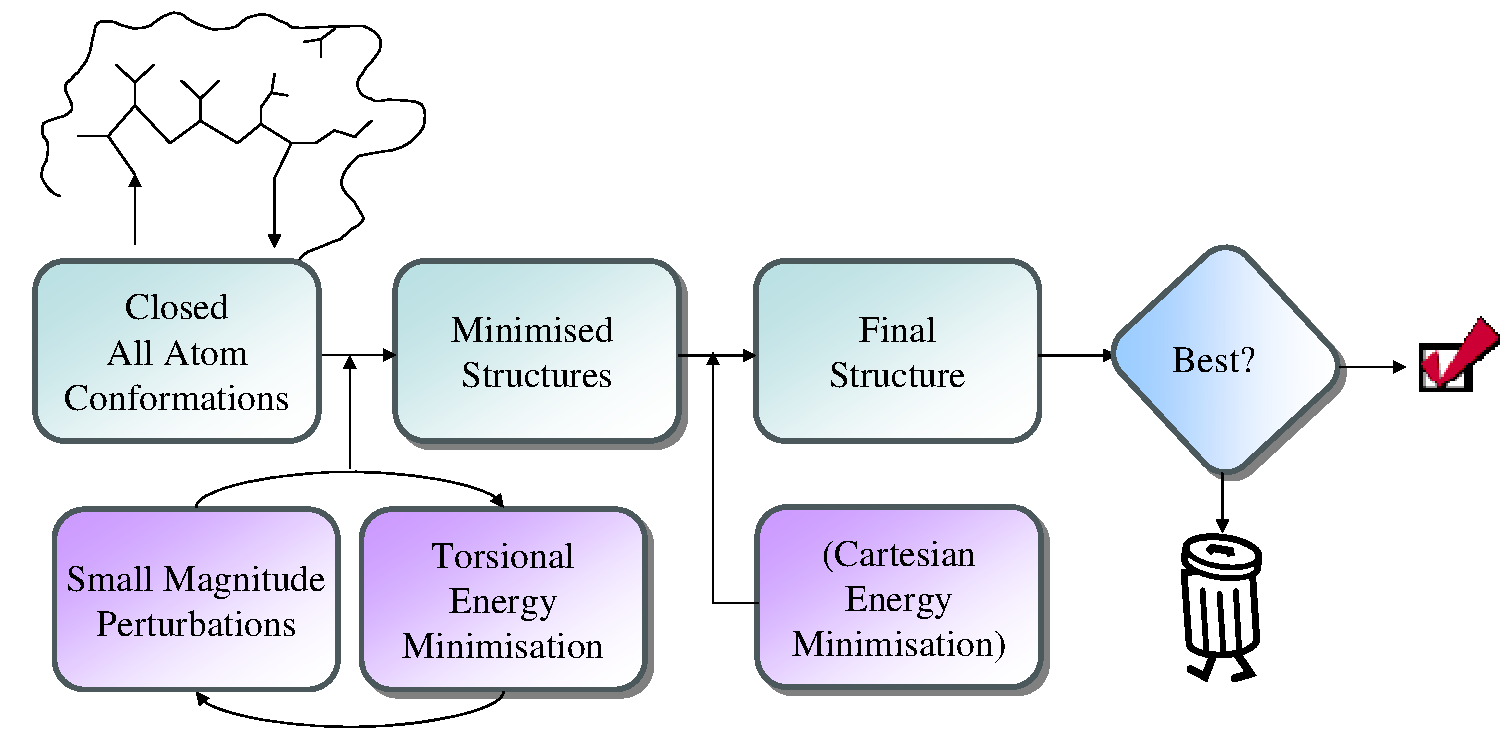
\includegraphics[width=0.9\textwidth]{./06-PreArcus/stage-3/stage-3.pdf}
\end{center}
\caption{The execution logic for \prearcus\ stage 3.}
\label{fig:prearcus:stage_3}
\end{figure}

\section{Discussion}

In this chapter, the refinement stages of \prearcus\ have been described in full. \prearcus\ exhibits a number of features that are not always found in other methods. The most simple of these is the fact that it produces all-atom models, whereas some other methods only produce \mainchain\ models\cite{METHOD:Petra}. Secondly, many methods neglect the cis \Omg-torsion angle and so are fundamentally incapable of modelling loops which contain them\cite{METHOD:CLOOP,METHOD:Plop,METHOD:Petra}. The use of  torsional energy-minimisation is unique amongst loop modelling methods and has been shown to be capable of finding lower energy-minima than Cartesian energy minimisation alone.
Finally,
it has been demonstrated that the \amberff\ forcefield
with the generalized Born solvation model identifies
near-native conformations significantly better than
previous methods\cite{METHOD:RapperA,METHOD:RapperB}.
Its use is therefore an important feature of \prearcus.

A second major advantage of \prearcus\ is that it is built upon the \pd\ molecular mechanics library. It, therefore, inherits all of the functionality from the library, as well as any future functionality and performance enhancements.
One of the most important aspects of this is that \prearcus\ can be executed with any of the \forcefields\ found in \pd.
This means that at a later date other molecular mechanics \forcefields\ such as \opls\ and \charmm\ may be assessed, as well as other statistical \forcefields\ which may be implemented within the framework.
The same is true of many other base-classes found in \pd, including perturbations, monitors, and structural filters. As perturbations are a key element of \prearcus, trials of alternative perturbation configurations, such as those including Cartesian movements can easily be implemented within \pd.
Finally, \pd's comprehensive restraint system can easily be applied to the candidate loop selection process. This allows scope for additional experimental information to be incorporated into the modelling process. Restraints from NMR, cross-linking, or strong homology information can all be applied with trivial additional effort.

The qualitative performance characteristics of \prearcus\ are assessed in chapter \ref{chapter:casp}. Following this, a quantitative performance analysis with respect to other methods in the literature is performed in chapter \ref{chapter:methods}.









